\chapter{ Le  Machine Learning}
\label{Le Machine Learning}
\thispagestyle{fancy}




\section{Généralités sur le Machine Learning}
\label{Le Machine Learning: Généralités sur le Machine Learning}
Le Machine Learning (traduire par apprentissage automatique) est une ramification de l'intelligence artificielle. Son champ d'étude est vaste et en perpétuelle évolution. Les solutions offertes par cette discipline permettent d'étudier toute sorte de données et d'automatiser une multitude de systèmes. L'apprentissage automatique rencontre un succès croissant qui est corrélé avec l'essor des nouvelles technologies et l'automatisation de l'analyse de volumes conséquents de données (Big Data). Les applications sont multiples, en voici quelques exemples:  

\begin{itemize}
	\item Algorithmes des moteurs de recherches (Google Deep Dream\cite{DeepDream}, Google TensorFlow \cite{TensorFlow})
	\item Analyse boursière
	\item Analyse de rapports d'erreurs
	\item Reconnaissance vocale, biométrie, reconnaissance d'écriture
	\item Robotique (vision, mouvements, prise de décision, etc.)
	\item Neurosciences 
\end{itemize}



\subsection{Définition et principes généraux du Machine Learning}
\label{Le Machine Learning: Généralités sur le Machine Learning: Définition et principe général}
Le champ d'étude et d'application du Machine Learning étant immense, on propose de redéfinir cette notion en l'adaptant à la résolution de notre problématique (i.e. automatiser l'analyse d'incidents révélés lors du filtering test).
On offre ici deux définitions de l'apprentissage automatique: une première dite "High Level" qui le caractérise de manière générale et une seconde qui reflète sa dimension algorithmique. 

\begin{description}
	\item[High Level]: Le Machine Learning permet à un système d'évoluer grâce à un processus d'apprentissage et ainsi de remplir des tâches qu'il est difficile, voire impossible, de remplir par d'autres moyens algorithmiques plus classiques. 
	\item[Mathématique] Le Machine Learning fourni les outils pour prédire une/des donnée(s) de sortie Y à partir des données d'entrée X via un processus d'apprentissage. 
\end{description}
 
Au regard des deux définitions stipulées ci-dessus, on peut représenter le principe de base de l'apprentissage automatique sous la forme d'un schéma bloc (figure \ref{fig:Schéma fonctionnel haut niveau du Machine Learning}).

\begin{figure}[h]
	\centering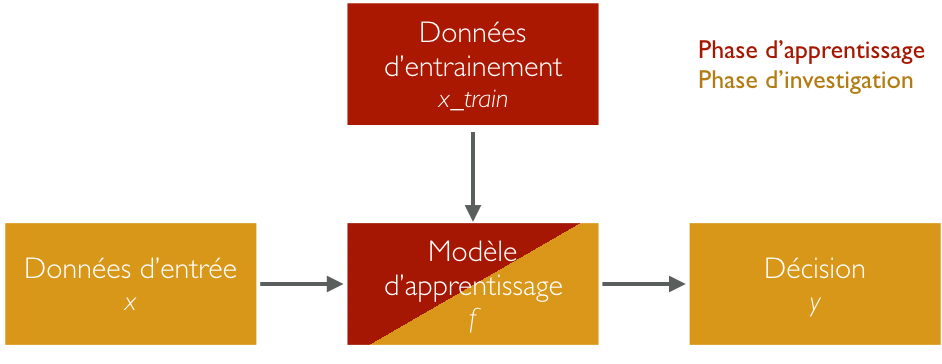
\includegraphics[height=5cm]{images/ML_high_level.png}
	\caption{Schéma fonctionnel haut niveau du Machine Learning}
	\label{fig:Schéma fonctionnel haut niveau du Machine Learning}
\end{figure}

L'apprentissage automatique peut être vu dans sa globalité comme un processus composé de deux étapes successives : 
\begin{enumerate}
		\item [Apprentissage]
		 \begin{enumerate}
			\item  Un ensemble de données est mis à l'entrée du système lors de la phase d'apprentissage ($x\_train$).
			\item A partir de ces informations, le système ($f$) apprend - s'entraîne- pour être en capacité de prendre une décision vis à vis de la tâche qui lui sera demandée. 
		\end{enumerate}
		
		\item [Prise de décision] 
		\begin{enumerate}
			\item  On a en entrée du système une ou des donnée(s) brutes ($x$).  
			\item Cette donnée est traitée et analysée par le système.
			\item En sortie, une décision ($y$) est prise quant à la tâche demandée grâce à l'apprentissage effectué en amont. 
		\end{enumerate}
\end{enumerate}


\subsubsection{Un exemple concret}
\label{Le Machine Learning: Généralités sur le Machine Learning: Définition et principe général:un exemple concret}
Afin d'exposer de manière plus concrète le processus fonctionnel haut niveau d'un algorithme d'apprentissage, on soumet l'exemple suivant:

\textit{On cherche à déterminer la période de l'année à laquelle on se trouve actuellement (i.e. printemps, été, automne ou hiver) grâce à l'analyse de l'humidité, la température et la pression atmosphérique d'aujourd'hui. \\
	La première étape est d'entraîner notre système afin que celui-ci soit en mesure de prendre une décision vis-à-vis des données qu'on lui présentera en entrée (i.e. l'humidité, la température et la pression atmosphérique d'aujourd'hui). \\
	Une fois le système entrainé, on attend de celui-ci ce type de comportement : \\
	On présente en entrée du système une température de -2\degres C, une pression atmosphérique de 1030hPa et un taux d'humidité de 81\%. La décision (sortie) espérée est: \emph{hiver}}.

On peut adapter le schéma fonctionnel haut niveau du Machine Learning à notre exemple figure \ref{fig:Schéma fonctionnel haut niveau du Machine Learning, exemple prévision saisonnière}. 

\begin{figure}[h]
	\centering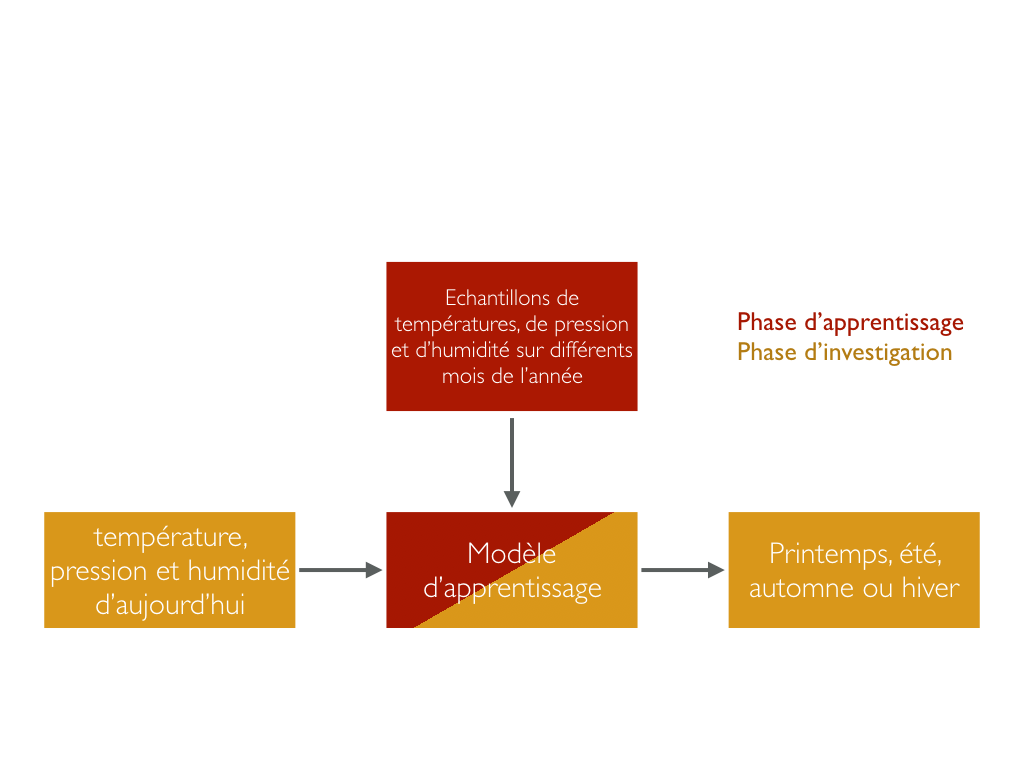
\includegraphics[height=5cm]{images/ML_high_level_expl.png}
	\caption{Schéma fonctionnel haut niveau du Machine Learning, l'exemple de la prévision saisonnière}
	\label{fig:Schéma fonctionnel haut niveau du Machine Learning, l'exemple prévision saisonnière}
\end{figure}

\subsubsection{Lexique} 
\label{Le Machine Learning: Généralités sur le Machine Learning: Définition et principe général:Lexique}
Pour caractériser et  désigner plus précisément les différents éléments de notre système, on présente ci-dessous le champs lexical rattaché au Machine Learning:

\begin{description}
	\item [Features] Le type de données présentées en entrée. \\
	\textit{La température, la pression atmosphérique et l'humidité.}
	\item [Echantillons ou exemples] Les données permettant d'entrainer le système ($x\_train$). \\
	\textit{Des échantillons de température, pression atmosphérique et humidité pris à différents périodes de l'année.}
	\item [Modèle d'apprentissage] Le cœur du système décisionnel ($f$).
	\item [Décision] La sortie ou réponse du système ($y$) \\
	\textit{Printemps, été, automne ou hiver.}
\end{description}



\subsection{Les exemples}
\label{Le Machine Learning: Généralités sur le Machine Learning: Les données}
Les exemples sont les données utilisées pour entraîner l'algorithme d'apprentissage. On parle également d'échantillons. Ils sont regroupés en "features" (terme anglais, traduire par caractéristiques). 
Pour reprendre l'exemple cité précédemment (partie \ref{Le Machine Learning: Généralités sur le Machine Learning: Définition et principe général:un exemple concret}), nos données sont regroupées en 3 features: la température, l'humidité et la pression atmosphérique. Les exemples sont donc structurés de la manière suivante: 

\begin{equation}
\begin{blockarray}{cccc}
& temperature (\degres C) & humidite (\%) & pression(HPa) \\
\begin{block}{c(ccc)}
Exemple_1 & -10 & 85 & 1023 \\
Exemple_2 & 15 & 80 & 1020 \\
Exemple_3 & 23 & 65 & 1015 \\
... & ... & ... & ... \\
Exemple_n & 10 & 81 &  1032 \\
\end{block}
\end{blockarray}
\label{exemples prévision saisonnière}
\end{equation}

\begin{equation}
\begin{blockarray}{cccc}
& temperature (\degres C) & humidite (\%) & pression(HPa) \\
\begin{block}{c(ccc)}
Exemple_1 & -10 & 85 & 1023 \\
Exemple_2 & 15 & 80 & 1020 \\
Exemple_3 & 23 & 65 & 1015 \\
... & ... & ... & ... \\
Exemple_n & 10 & 81 &  1032 \\
\end{block}
\end{blockarray}
\end{equation}


\subsubsection{Différents types d'exemples}
\label{Le Machine Learning: Généralités sur le Machine Learning: Les données: Différents types d'exemples}
Il existe deux types de données: les échantillons labellisés et non labellisés.

Pour reprendre l'exemple de la prévision saisonnière (partie \ref{Le Machine Learning: Généralités sur le Machine Learning: Définition et principe général:un exemple concret}), on a les jeux de données suivants: 

\paragraph{Données labellisées} 
Les échantillons labellisés correspondent à des exemples corrélés à une sortie - un label - connue.
\begin{equation}
\begin{blockarray}{ccccc}
& température (\degres C) & humidite (\%) & pression(HPa) \\
\begin{block}{c(ccc)c}
Exemple_1 & -10 & 85 & 1023 & hiver\\
Exemple_2 & 15 & 80 & 1020 & automne\\
Exemple_3 & 23 & 65 & 1015 & ete \\
... & ... & ... & ... \\
Exemple_n & 10 & 81 &  1032 & printemps\\
\end{block}
\end{blockarray}
\end{equation}
On connait la sortie qui correspond aux données d'entrée, i.e. que on sait à quelle période de l'année les échantillons ont été prélevé.
 
\paragraph{Données non labellisées} 
Les échantillons non labellisés ne sont quant à eux pas corrélés à une sortie. 
\begin{equation}
\begin{blockarray}{ccccc}
& température (\degres C) & humidite (\%) & pression(HPa) \\
\begin{block}{c(ccc)c}
Exemple_1 & -10 & 85 & 1023 & ??\\
Exemple_2 & 15 & 80 & 1020 & ??\\
Exemple_3 & 23 & 65 & 1015 & ?? \\
... & ... & ... & ... \\
Exemple_n & 10 & 81 &  1032 & ??\\
\end{block}
\end{blockarray}
\end{equation}
On ne connait pas la sortie qui correspond aux données d'entrée, i.e. on \emph{ne} sait \emph{pas} à quelle période de l'année les échantillons ont été prélevés. 



\subsection{La décision}
\label{Le Machine Learning: Généralités sur le Machine Learning: La décision}
La décision correspond à la sortie du système, i.e. le choix réalisé par l'algorithme d'apprentissage automatique vis-à-vis de la tâche qui lui a été confié.

\subsubsection{Différents types de sorties}
\label{Le Machine Learning: Généralités sur le Machine Learning: La décision: Différents types de sorties}
Il existe différents types de sortie: les sorties continues et discrètes.

\begin{description}
	\item [Sorties continues] peuvent prendre n'importe quelle valeur. \\
	 $y \in R$ \\
	 \textit{Déterminer l'évolution de la température en fonction des échantillons enregistrés les mois précédents correspond à une sortie continue.}
	\item [Sorties discrètes] ne peuvent prendre que des valeurs prédéterminées. \\
	 $y \in {1, 2, 3, ...,C}$ \\
	\textit{ L'exemple partie \ref{Le Machine Learning: Généralités sur le Machine Learning: Définition et principe général:un exemple concret} a une sortie discrète. En effet, la sortie ne peut prendre que des valeurs prédéterminées: printemps, été, automne et hiver.}
\end{description}



\subsection{Le modèle}
\label{Le Machine Learning: Généralités sur le Machine Learning: Le modèle}
Il existe différents types d'apprentissages. Le choix d'un modèle en particulier est influencé par le type d'exemples que l'on a en entrée du système et du type de décision que l'on souhaite obtenir en sortie. Nous nous intéresserons à différentes catégories d'apprentissages automatiques.

\subsubsection{Apprentissage supervisé et non supervisé} 
\label{Le Machine Learning: Généralités sur le Machine Learning: Le modèle: apprentissage supervisé et non supervisé}
L'apprentissage supervisé nécessite d'avoir des données labellisées en entrée, i.e. on connait le type de décision que l'on aura en sortie du système, en fonction des exemples en entrée: il y'a une corrélation entre la sortie et l'entrée. C'est cette notion qui s'exprime au travers du terme \emph{supervisé}. 
L'apprentissage non supervisé s'appuie quant à lui sur l'utilisation d'une base de donnée non labellisée pour son apprentissage, i.e qu'on ne connait pas le type de décision associé aux exemples en entrée. Dans le cas d'un apprentissage non supervisé, pour parvenir à prendre une décision, l'algorithme devra diviser les groupes de données hétérogènes en sous-groupes homogènes d'informations, ayant des caractéristiques similaires. On appelle ces subdivisions des \emph{clusters}.
Afin de matérialiser les différences entres les deux méthodes et les applications possibles pour chacune d'elles, on propose deux exemples tableau \ref {tab: Comparaison des différentes méthodes d'apprentissage}.

\begin{table}[H]
	\begin{tabular}{ | p {2.5cm} | p {6cm} | p {6cm} |}
	\hline
	 & apprentissage supervisé & apprentissage non supervisé \\
	\hline
	\begin{tabular}{c} exemple n\degres1:\\apprendre aux \\ humains \end{tabular}  &
	 Une institutrice enseigne à ses élèves à différencier un chat d'un chien: c'est la décision qu'on attend d'eux. Pour cela, l'éducatrice leur montre différentes photographies de chiens et de chats: ce sont les exemples utilisés pour l'apprentissage. Ces exemples peuvent être segmentés en différentes caractéristiques, comme la taille de l'animal, sa couleur, la longueur du poil, etc: il s'agit des features. Lorsque l'institutrice leur présente les différentes images, elle stipule clairement si il s'agit d'un chien ou d'un chat: il y'a donc une corrélation entre l'entrée et la sortie de l'apprentissage, il s'agit d'un apprentissage supervisé (figure \ref{fig:Comparaison d'un apprentissage supervisé et non supervisé dans le cadre de l'exemple "apprendre aux humains"},a).&
	 Une institutrice donne à ses élèves le même exercice que dans le cadre de l'apprentissage supervisé, à la différence que lorsqu'elle présente les différentes images, elle \emph{ne} stipule \emph{pas} la race de l'animal: il n'y a donc aucune corrélation entre l'entrée et la sortie de l'apprentissage, il s'agit donc d'un apprentissage non supervisé. Pour réussir cet exercice, les enfants devront donc regrouper les animaux en s'appuyant sur leurs similitudes physiques, i.e. leurs features (e.g. taille de l'animal, sa couleur, longueur du poil, etc.). Les élèves ne connaitront certes pas le nom des deux animaux, mais ils auront su les différencier. C'est la même approche qui est mis en œuvre en apprentissage automatique non supervisé (figure \ref{fig:Comparaison d'un apprentissage supervisé et non supervisé dans le cadre de l'exemple "apprendre aux humains"}, b). \\
	\hline 
	\begin{tabular}{c} exemple n\degres2:\\prévisions \\saisonnières \\ \ref{Le Machine Learning: Généralités sur le Machine Learning: Définition et principe général:un exemple concret}\end{tabular} &
	On reprend l'exemple dans lequel on souhaite prendre une décision quant à la période de l'année à laquelle on se trouve actuellement, en fonction des features humidité, température et pression atmosphérique. On prélève des échantillons à différentes périodes de l'année en notant à quelle saison ces données ont été prélevées: ce sont des exemples labellisés, i.e. il y'a une corrélation entre les données et la sortie du système. Il s'agit donc d'un apprentissage supervisé (figure \ref{fig:Comparaison d'un apprentissage supervisé et non supervisé dans le cadre de l'exemple prévision saisonnières}, a). &
	Cette fois-ci on ne note pas la saison à laquelle les échantillons ont été prélevés. Pour résoudre le problème, l'algorithme doit donc associer les données les plus similaires entre elles et ainsi créer des groupes homogènes d'informations qui correspondront aux 4 décisions possibles (figure \ref{fig:Comparaison d'un apprentissage supervisé et non supervisé dans le cadre de l'exemple prévision saisonnières}, b). \\
	\hline
	\end{tabular}
	\caption[Comparaison des différents modèles d'apprentissage]{Comparaison de l'apprentissage supervisé et non supervisé par des exemples}
	\label {tab: Comparaison des différentes méthodes d'apprentissage}
\end{table}

\begin{figure}[H]
	\centering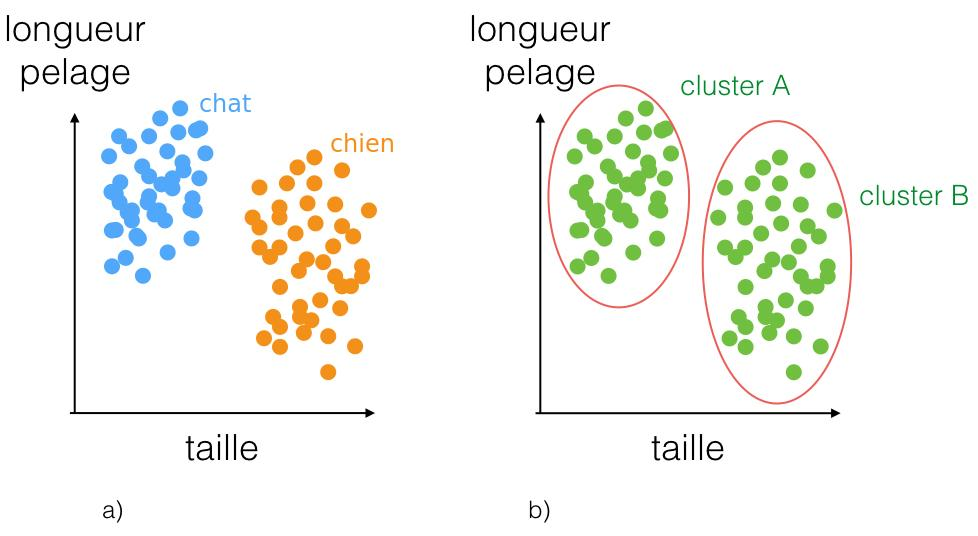
\includegraphics[height=7cm]{images/apprentissage_chat.jpeg}
	\caption[Comparaison d'un apprentissage supervisé et non supervisé dans le cadre de l'exemple "apprendre aux humains"]{Comparaison d'un apprentissage supervisé et non supervisé dans le cadre de l'exemple "apprendre aux humains". On observe sur la figure a) les différents exemples d'entrainement exprimés dans un repère composé des deux features "taille" et "longueur de pelage". On remarque qu'il y a la formation de deux groupes de données homogènes: les animaux de taille globalement élevée avec un pelage court et les animaux de taille moindre avec un poil globalement plus long. Les données étant labellisées, on sait que le premier groupe correspond à des chiens et le deuxième à des chats. Dans le cas de la figure b), les exemples n'étant pas labellisés, l'algorithme ne peut pas regrouper les données en fonction de leurs valeurs de sortie. Il réunit donc les ensembles homogènes de données en clusters.}
	\label{fig:Comparaison d'un apprentissage supervisé et non supervisé dans le cadre de l'exemple "apprendre aux humains"}
\end{figure}

\begin{figure}[H]
	\centering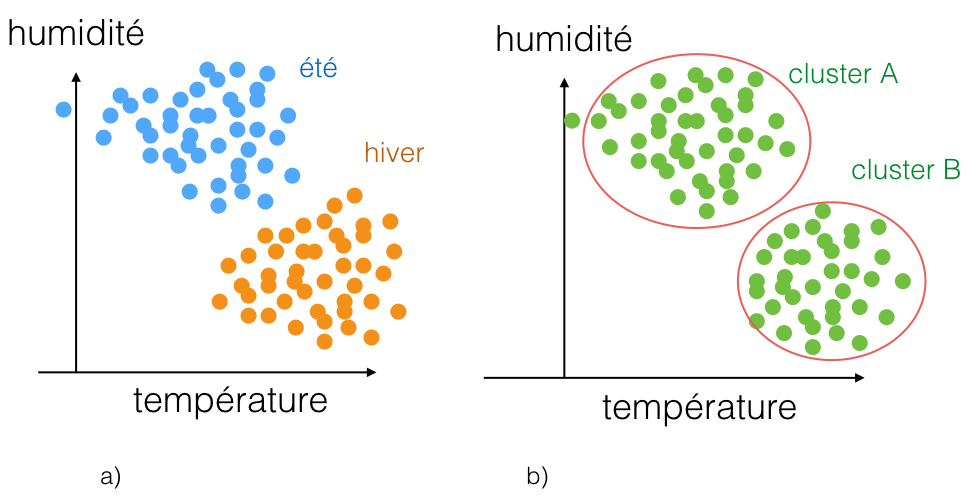
\includegraphics[height=7cm]{images/apprentissage_meteo.jpeg}
	\caption[Comparaison d'un apprentissage supervisé et non supervisé dans le cadre de l'exemple "prévisions saisonnières"]{Comparaison d'un apprentissage supervisé et non supervisé dans le cadre de l'exemple "prévisions saisonnières". On observe sur la figure a) les différents exemples d'entrainement exprimés dans un repère composé des deux dimensions (features) "humidité" et "température". On remarque qu'il y a la formation de deux groupes de données homogènes: un où les échantillons sont prélevés lors de saisons globalement chaudes et sèches, l'autre où les échantillons sont enregistrés lors de périodes globalement froides et humides. Les données étant labellisées, on sait que le premier groupe correspond à l'été et l'autre groupe à l'hiver. Dans le cas de la figure b), les exemples n'étant pas labellisés, l'algorithme ne peut pas regrouper les données en fonction de leurs valeurs de sortie. Il réunit donc les ensembles homogènes de données en clusters.}
	\label{fig:Comparaison d'un apprentissage supervisé et non supervisé dans le cadre de l'exemple prévision saisonnières}
\end{figure}

Il existe deux types d'apprentissage supervisé: la régression et la classification.


\subsubsection{Apprentissage supervisé: régression et classification} 
\label{Le Machine Learning: Généralités sur le Machine Learning: Le modèle:Regression et classification}
 La régression est un type d'apprentissage avec lequel on souhaite obtenir une sortie continue. Dit de manière différente, la régression implique le fait que l'on souhaite \emph{estimer} ou \emph{prédire} une réponse. La classification est quant à elle un type d'apprentissage avec lequel on souhaite obtenir une sortie discrète. Elle peut être vue comme un cas particulier de la régression, où les valeurs à prédire sont discrètes. Formulé autrement, la classification implique le fait que l'on souhaite \emph{classer} un exemple parmi différentes catégories. 
 \newline
 Afin de mettre en avant les nuances qui existent entre les deux méthodes et les applications possibles pour chacune d'elle, on propose l'exemple tableau \ref {tab: Comparaison des différentes catégories d'apprentissage supervisé}).

\begin{table}[H]
	\begin{tabular}{ | p {7cm} | p {7cm} |}
		\hline
		régression & classification \\
		\hline
		On souhaite connaitre le temps (température et humidité) qu'il fera pendant les jours suivants. Pour cela, on s'appuie sur les différents échantillons de température et d'humidité enregistrés lors des mois et des années précédentes (exemples labellisés). Le fait de déterminer la température des jours suivants relève de la prédiction (figure \ref {tab: Comparaison des différentes catégories d'apprentissage supervisé}, a).  
		 &  L'exemple de la prédiction saisonnière \ref{Le Machine Learning: Généralités sur le Machine Learning: Définition et principe général:un exemple concret} est un problème de classification: on cherche à classer notre donnée d'entrée parmi plusieurs groupes de données homogènes: printemps, été automne ou hiver (figure \ref {tab: Comparaison des différentes catégories d'apprentissage supervisé}, b). \\
		\hline 
	\end{tabular}
	\caption[Comparaison des différentes catégories d'apprentissage supervisé]{Comparaison entre l'apprentissage supervisé de type régression et supervisé de type classification}
	\label {tab: Comparaison des différentes catégories d'apprentissage supervisé}
\end{table}

\begin{figure}[h]
	\centering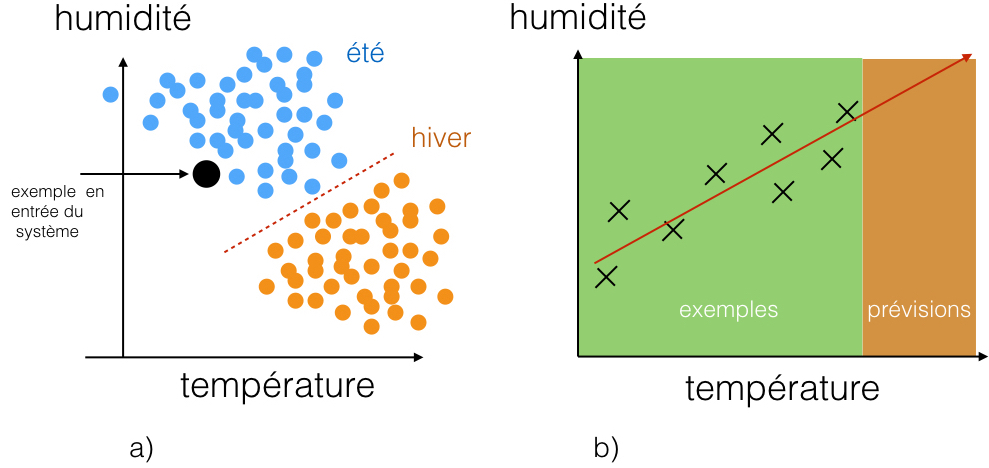
\includegraphics[height=6.5cm]{images/regression_class.jpeg}
	\caption[Comparaison par l'exemple de la régression et de la classification]{Comparaison par l'exemple de la régression et la classification. Sur la figure a), on observe deux jeux de données homogènes (été et hiver) qui s'expriment dans un repère en deux dimensions (features humidité et température). Le but est ici de classer l'exemple en entrée du système parmi ces deux classes. Il s'agit donc d'un problème de classification. Dans la figure b), on observe une succession d'exemples exprimés dans un repère en deux dimensions (features température et humidité). On remarque une évolution globalement linéaire de ces exemples, nous permettant ainsi de prédire la température et l'humidité sur les prochains mois: il s'agit d'un problème de régression.}
	\label{fig:Comparaison par l'exemple de la régression et la classification}
\end{figure}





\section{Les différents algorithmes d'apprentissage supervisé}
\label{Le Machine Learning:Les différents algorithmes d'apprentissage supervisé}
Il existe différents algorithmes d'apprentissage supervisé utilisés pour résoudre des problèmes de régression et de classification. 


\subsection{La régression linéaire uni-variable}
\label{Le Machine Learning:Les différents algorithmes d'apprentissage supervisé: La regression linéaire}
La régression linéaire cherche à expliquer une variable de sortie $y$ par une fonction affine de $x$. Cette fonction linéaire affine est appelée \emph{hypothèse} (notée $h(x)$). Dit de manière différente : on a un jeu de données $x$ auquel correspond un jeu de données $y$, on cherche les valeurs $\theta_1$ et $\theta_2$ permettant de "mapper" les données, tel que:

\begin{equation}
	h_\theta (x) = \theta_0 + \theta_1 x
\end{equation}


\subsubsection{Exemple de régression linéaire uni-variable}
\label{Le Machine Learning:Les différents algorithmes d'apprentissage supervisé: La regression linéaire: Exemple de régression linéaire uni-variable}
On souhaite déterminer le prix d'un logement en fonction de sa surface au sol en se basant sur les exemples de prix du parc immobilier. 
La surface au sol est donc l'entrée $x$ de notre système et le prix la sortie $y$. A partir des exemples du tableau \ref {tab:parc immobilier}, on obtient la représentation graphique en figure \ref{fig:évolution du prix de l'immobilier en fonction de la surface}. Grâce à l'expression de l'hypothèse, on est capable de déterminer le prix d'un loyer en fonction de la surface au sol.  

\begin{table}[H]
	\begin{tabular}{ | p {4cm} | p {4cm} |}
		\hline
		taille ($m^2$) & prix (k\euro) \\
		\hline
		2104 & 460 \\
		1416 & 232 \\
		1534 & 314 \\
		852 & 178 \\
		500 & 100 \\ 
		1012 & 212 \\
		126 & 75 \\
		1775 & 432 \\
		600 & 150 \\
		2114 & 510 \\
		1316 & 270 \\
		1634 & 334 \\
		\hline 
	\end{tabular}
	\caption[parc immobilier]{exemples de prix des logements en fonction de leur taille}
	\label {tab:parc immobilier}
\end{table}

\begin{figure}[h]
	\centering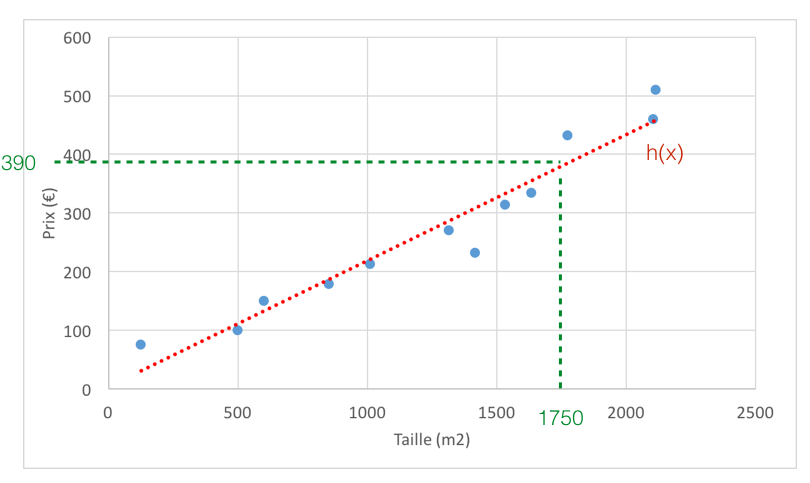
\includegraphics[height=8cm]{images/graph_immobilier.png}
	\caption[Évolution du prix de l'immobilier en fonction de la surface]{Évolution du prix de l'immobilier en fonction de la surface. L'ensemble des données semblent globalement évoluer de manière linéaire. Cette linéarité est représentée par l'hypothèse $h(x)$. Grâce à celle-ci, on peut déterminer le prix d'un logement en fonction de sa superficie, et inversement. Par exemple, un appartement d'une surface de 1750 $m^2$ coutera aux alentours de 390k\euro.}
	\label{fig:Évolution du prix de l'immobilier en fonction de la surface}
\end{figure}

Cet exemple est dit uni-variable car un seul jeu de données $x$ (superficie) correspond à un jeu de données $y$ (prix).


\subsubsection{La fonction coût}
La fonction coût (en anglais cost function) compare la moyenne des différences entre les résultats de l'hypothèse $h(x)$ et les sorties actuelles $y$. Cela signifie qu'elle cherche à minimiser les valeurs calculées via l'hypothèse et les valeurs réelles (cf. figure \ref{fig:Régression linéaire, optimisation de la fonction coût}). 
Soit: 

\begin{equation}
	J(\theta_0,\theta_1) = \frac{1}{2m}\sum_{i=1}^{m}(h_\theta(x^i)-y^i)^2
\end{equation}

avec:
\begin{itemize}
	\item $J(\theta_0,\theta_1)$ la fonction coût
	\item $\theta_0$ et $\theta_1$ les paramètres de l'hypothèse $h(x)$
	\item $m$ le nombre d'exemples disponibles pour l'entrainement 
	\item $h_\theta(x)$ l'hypothèse $h_\theta (x) = \theta_0 + \theta_1 x$
	\item $x^i$ exemple $i$
	\item $y^i$ sortie $i$
\end{itemize}

\begin{figure}[h]
	\centering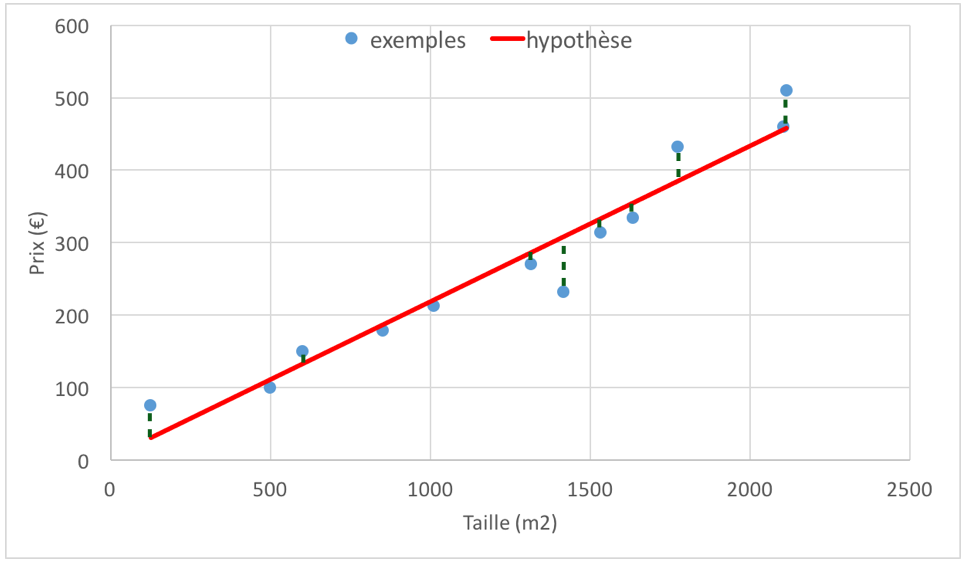
\includegraphics[width=12cm]{images/cost.png}
	\caption[Régression linéaire, optimisation de la fonction coût]{Régression linéaire, optimisation de la fonction coût. Le calcul de la fonction coût revient à minimiser la distance entre un exemple et l'hypothèse, et ce pour chaque exemple.}
	\label{fig:Régression linéaire, optimisation de la fonction coût}
\end{figure}


\subsubsection{Algorithme du gradient}
On cherche à minimiser la valeur de la fonction coût $J(\theta_0,\theta_1)$ en jouant sur les paramètres $\theta_0$ et $\theta_1$ de l'hypothèse. Pour cela, on calcule la fonction coût pour différentes valeurs de $\theta_0$ et $\theta_1$ et on cherche la valeur minimale de $J(\theta_0,\theta_1)$. Dans l'idée, cela revient à choisir une valeur de $\theta$ et de "faire un pas" vers la direction la plus basse, il s'agit d'un calcul itératif. La forme de la courbe $J$ en fonction de  $\theta_0$ et $\theta_1$ étant convexe (cf. figure \ref{fig:Régression linéaire, calcul des paramètres de l'hypothèse}), cela revient à trouver le minimum global de la courbe en appliquant l'algorithme du gradient (en anglais, gradient descent):

\begin{equation}
	\begin{split}
		\text{repeat: \{} \\
		\theta_0 = \theta_0 - \alpha \frac{\partial J(\theta_0,\theta_1)}{\partial\theta_0} \\
		\theta_1 = \theta_1 - \alpha \frac{\partial J(\theta_0,\theta_1)}{\partial\theta_1} \\
		\text{\}}
	\end{split}
\end{equation}

avec $\alpha$ la taille du "pas" que l'on fait vers la direction la plus basse. Si la valeur de $\alpha$ est trop petite, le nombre d'itération sera plus important, augmentant ainsi le temps de calcul. Si la valeur de $\alpha$ est trop grande, on risque de ne pas pouvoir atteindre le minimum et de diverger.  

\begin{figure}[h]
	\centering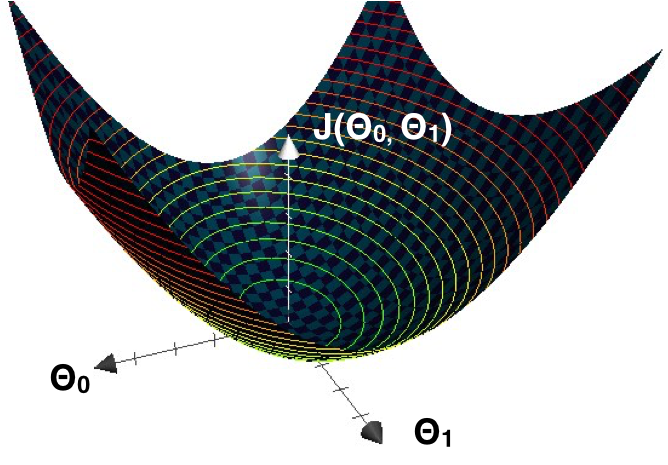
\includegraphics[height=7cm]{images/gradient.png}
	\caption[Régression linéaire, calcul des paramètres de l'hypothèse]{Régression linéaire, calcul des paramètres de l'hypothèse. Ce graphique représente la variation des paramètres $\theta_0$ et $\theta_1$ de l'hypothèse en fonction de la valeur de la fonction coût. On cherche les valeurs  $\theta_0$ et $\theta_1$ minimisant $J(\theta_0,\theta_1)$. La courbe ayant la forme d'une "cuvette", les valeurs optimales de $\theta_0$ et $\theta_1$ correspondent à celles au fond de la "cuvette".}
	\label{fig:Régression linéaire, calcul des paramètres de l'hypothèse}
\end{figure}
 
 
 
\subsection{La régression linéaire multi-variable}
\label{Le Machine Learning:Les différents algorithmes d'apprentissage supervisé: La regression linéaire multi-variable}
On peut réaliser de la régression linéaire avec plusieurs features en entrée.


\subsubsection{Exemple de régression linéaire multi-variable}
\label{Le Machine Learning:Les différents algorithmes d'apprentissage supervisé: La regression linéaire multi-variable: Exemple de régression linéaire multi-variable}
Afin de présenter ce qu'est la régression linéaire multi-variable, on ajuste l'exemple partie \ref{Le Machine Learning:Les différents algorithmes d'apprentissage supervisé: La regression linéaire: Exemple de régression linéaire uni-variable} pour qu'il corresponde à un problème multi-variable.
 
On souhaite cette fois-ci déterminer le prix d'un logement en fonction de sa surface au sol, du nombre de pièces et du nombre d'étages, en se basant sur les exemples de prix du parc immobilier. On a donc plusieurs entrées (surface, nombre de pièces, nombre d'étages). Soit le tableau \ref {tab:parc immobilier multi}, les exemples $x$ utilisés pour l'entrainement.
\begin{table}[H]
	\begin{tabular}{ | p {4cm} | p {4cm} |}
		\hline
		taille ($m^2$) & prix (k\euro) \\
		\hline
		2104 & 460 \\
		1416 & 232 \\
		1534 & 314 \\
		852 & 178 \\
		500 & 100 \\ 
		1012 & 212 \\
		126 & 75 \\
		1775 & 432 \\
		600 & 150 \\
		2114 & 510 \\
		1316 & 270 \\
		1634 & 334 \\
		\hline 
	\end{tabular}
	\caption[parc immobilier multi-variable]{exemples du prix des logements en fonction de leur surface, du nombre d'étages et du nombre de pièces}
	\label {tab:parc immobilier multi}
\end{table}

\subsubsection{Généralisation de la fonction coût}
\label{Le Machine Learning:Les différents algorithmes d'apprentissage supervisé: La regression linéaire multi-variable: Généralisation de l'hypothèse}
La fonction hypothèse s'exprime sous cette forme: 

\begin{equation}
	h_\theta(x) = \theta_0 + \theta_1X_1 + \theta_2X_2 + \theta_3X_3
\end{equation}

Où $X_1$, $X_2$ et $X_3$ correspondent respectivement aux features surface, nombre d'étages et nombre de pièces.

On peut la généraliser sous cette forme : 

\begin{equation}
h_\theta(x) = \theta_0 + \theta_1X_1 + \theta_2X_2 + \theta_3X_3 + ... + \theta_nX_n
\label{hypotesis multivar}
\end{equation}


\subsubsection{Généralisation de la fonction coût}
\label{Le Machine Learning:Les différents algorithmes d'apprentissage supervisé: La regression linéaire multi-variable: Généralisation de la fonction coût}
On peut généraliser la fonction coût et l'utiliser pour l'appliquer à un problème de régression linéaire multi-variable, tel que :

\begin{equation}
J(\theta_1,\theta_2,\theta_3,...,\theta_n) =  \frac{1}{2m}\sum_{i=1}^{m}(h_\theta(x^i)-y^{i})^2
\end{equation}


\subsubsection{Généralisation de l'algorithme du gradient}
\label{Le Machine Learning:Les différents algorithmes d'apprentissage supervisé: La regression linéaire multi-variable: Généralisation de l'algorithme du gradient}
On peut généraliser l'algorithme du gradient utilisé lors de la régression linéaire uni-variable pour l'appliquer à un problème de régression linéaire multi-variable:
 
\begin{equation}
\begin{split}
\text{Repeat \{} \\
\theta_j = \theta_j - \alpha \frac{\partial J(\theta_0, \theta_1, \theta_2, \theta_3, ... , \theta_n)}{\partial\theta_j} \\
\text{\}} \\
\end{split}
\end{equation}

On met à jour simultanément l'ensemble des valeurs de $\theta$ lors de chaque itération. 
\begin{equation}
\begin{split}
\text{Repeat \{} \\
\theta_j = \theta_j - \alpha \frac{1}{m}\sum_{m}^{i=1}(h_\theta(x^i) - y^i)x_j^i \\
\text{\}} \\
\end{split}
\label{gradient descent multivar}
\end{equation}

avec $x_j^i$ l'entrée $j$ de l'entrainement $i$.


\subsubsection{Vectorisation des calculs}
\label{Le Machine Learning:Les différents algorithmes d'apprentissage supervisé: La regression linéaire multi-variable: Vectorisation des calculs}
On peut exprimer les exemples en entrée du système sous forme vectorielle: 

\begin{equation}
\begin{blockarray}{[c]}
X_0 \\
X_1 \\
X_2 \\
... \\
X_n 
\end{blockarray} = X
\end{equation}

De même, on réécrit les paramètres $\theta$ de l'hypothèse sous forme vectorielle:

\begin{equation}
\begin{blockarray}{[c]}
\theta_0 \\
\theta_1 \\
\theta_2 \\
... \\
\theta_n 
\end{blockarray} = \theta
\end{equation}

On peut alors réécrire l'hypothèse (équation \eqref{hypotesis multivar}):
\begin{equation}
	h_\theta(x) = \theta^TX
\end{equation}

L'algorithme du gradient (équation \eqref{gradient descent multivar}) s'exprime donc sous sa nouvelle forme vectorielle: 
\begin{equation}
\theta = \theta - \frac{\alpha}{m}\sum_{i=1}^{m}(h_\theta(x^i)-y^i)X^i
\end{equation}

\subsection{La régression logistique}
\label{Le Machine Learning: Les différents algorithmes: La regression logistique}
La régression logistique permet de résoudre des problèmes de classification. Elle découle de la régression linéaire et s'appuie sur les mêmes concepts.
On cherche à séparer des groupes de données homogènes dans un ensemble hétérogène. 

\subsubsection{Régression linéaire et classification}
\label{Le Machine Learning: Les différents algorithmes: La regression logistique: Régression linéaire et classification}
On reprend l'exemple de la prévision saisonnière en partie \ref{Le Machine Learning: Généralités sur le Machine Learning: Définition et principe général:un exemple concret} et on utilise de la régression linéaire afin de classer automatiquement l'échantillon qu'on lui présente en entrée dans une des classes printemps ou hiver, en fonction de la température (figure \ref{fig:Classification via regression linéaire}). 
Pour cela, on met en place un seuil de classification:
\begin{itemize}
	\item Si $h_\theta(x) > 0,5$ alors $y=1$
	\item Si $h_\theta(x) < 0,5$ alors $y=0$
\end{itemize}

Où $y = 0$ correspond à la période hiver et $y = 1$ l'été. 

\begin{figure}[h]
	\centering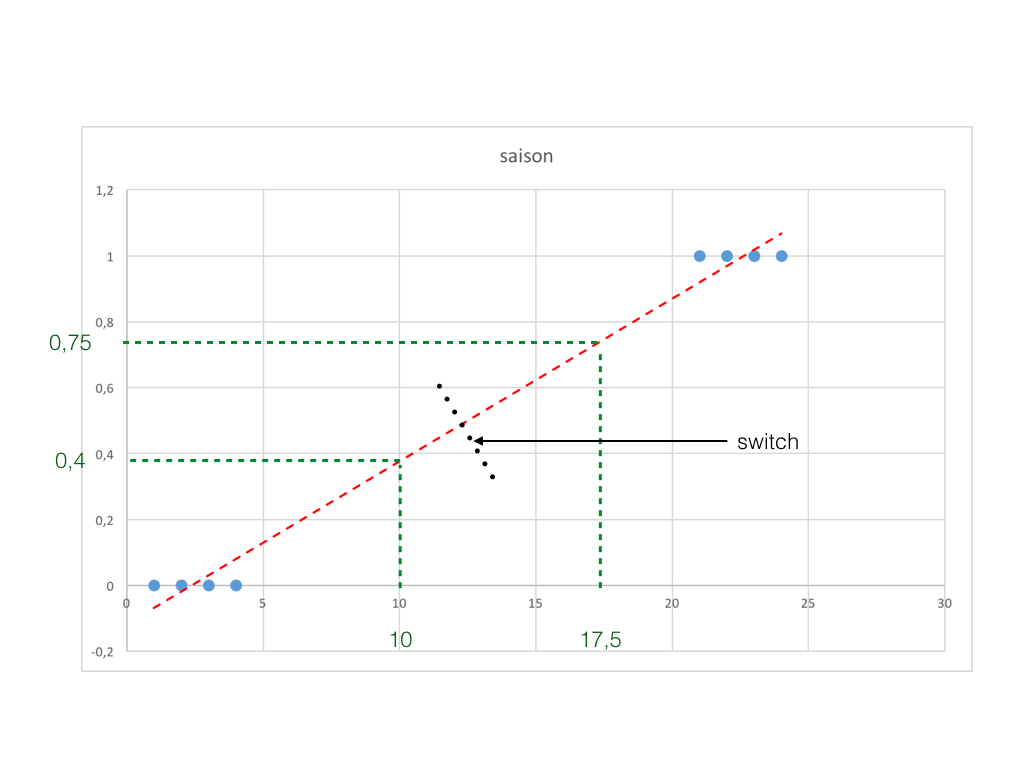
\includegraphics[height=5.5cm]{images/class_reg_lineaire.png}
	\caption[Classification via régression linéaire]{Classification via régression linéaire. On observe sur la figure a) que lorsque la température est inférieure à 12,5\degres C, le système considère que la valeur de sortie est 0 (hiver). Lorsque la température est au dessus, la valeur de sortie devient 1 (été). Ce cas particulier fonctionne car les exemples sont répartis de manière uniforme. Or, dans le cas de la figure b), on remarque qu'une répartition non uniforme des données entraîne un dysfonctionnement du classement. En effet, le seuil de différentiation entre les deux classes se situe aux alentours de  15\degres C, ce qui n'est pas représentatif des exemples.}
	%Reprendre ici avec de meilleurs arguments...
	\label{fig:Classification via regression linéaire}
\end{figure}

Cette méthode fonctionne dans le cas présent car les exemples sont régulièrement espacés entres eux. Dans le cas contraire, le seuil serait alors mal positionné et la classification serait erronée. La régression linéaire n'est donc pas adaptée pour la résolution de problèmes de classification. 

\subsubsection{Régression logistique et fonction sigmoïde}
\label{Le Machine Learning: Les différents algorithmes: La regression logistique: Régression logistique et fonction sigmoïde}
Pour réaliser de la classification en utilisant de la régression,  on peut modifier la forme linéaire de l'hypothèse en une sigmoïde (figure \ref{fig:Fonction sigmoïde}). On appelle également cette courbe fonction logistique ou fonction de répartition. D'un point de vue probabiliste, cela signifie que l'hypothèse représente la probabilité estimée que la sortie y soit égale à 1. Par exemple, si $h_\theta(x)=0,7$ signifie que l'on a 70\% de chance que la variable de sortie soit égale à 1.  

avec $g(x) = \frac{1}{1 + e^{-z}}$  la fonction sigmoïde, on a l'hypothèse $h_\theta(x)$ suivante: 
\begin{equation}
	h_\theta(x)=g(\theta^Tx) 
\end{equation}

soit: 
\begin{equation}
h_\theta(x)=\frac{1}{1 + e^{\theta^Tx}} 
\end{equation}

\begin{figure}[h]
	\centering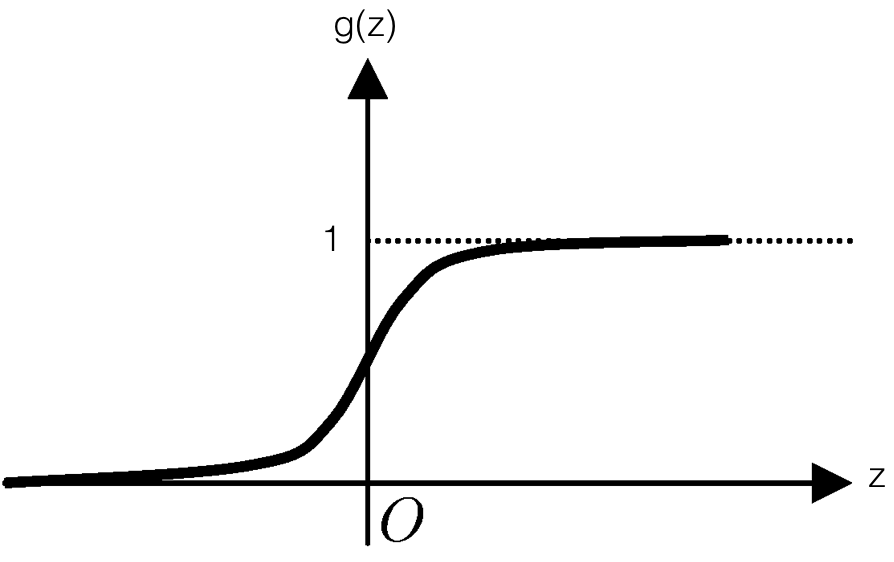
\includegraphics[height=5cm]{images/sigmoid.png}
	\caption[Fonction sigmoïde]{Fonction sigmoïde, également appelée fonction logistique.}
	%Reprendre ici avec de meilleurs arguments...
	\label{fig:Fonction sigmoïde}
\end{figure}

\subsubsection{Ligne de décision}
\label{Le Machine Learning: Les différents algorithmes: La regression logistique: Ligne de décision}
On a la propriété de la fonction sigmoïde suivante: 
\begin{equation}
 g(z) \ge 0,5 \text{ lorsque } z \ge 0
\end{equation}

On a donc pour l'hypothèse la propriété suivante: 
\begin{equation}
h(x)=g(\theta^Tx) \ge 0,5 \text{ lorsque } \theta^Tx \ge 0
\end{equation}

On peut alors émettre les deux affirmations suivantes:
\begin{equation}
	\begin{split}
	y=1 \text{ si }h_\theta(x) \ge 0,5 \text{ , soit } \theta^Tx \ge 0 \\
	y=0 \text{ si }h_\theta(x) \le 0,5 \text{ , soit } \theta^Tx \le 0 
	\end{split}
\end{equation}

\paragraph{application:}
Soit $h_\theta(x) = g(\theta_0 + \theta_1x_1 + \theta_2x_2)$ avec $\theta = \begin{blockarray}{[c]} -3 \\ 1 \\ 1 \end{blockarray}$, on a la condition suivante :
\begin{equation}
	y=1 \text{ si } -3 + x_1 + x_2 \ge 0 \text{ , soit } x_1 + x_2 \ge 3
\end{equation}

Cette expression correspond à la ligne (ou frontière) de décision de la régression linéaire (figure \ref{fig:Exemple d'une regression logistique}).

\begin{figure}[h]
	\centering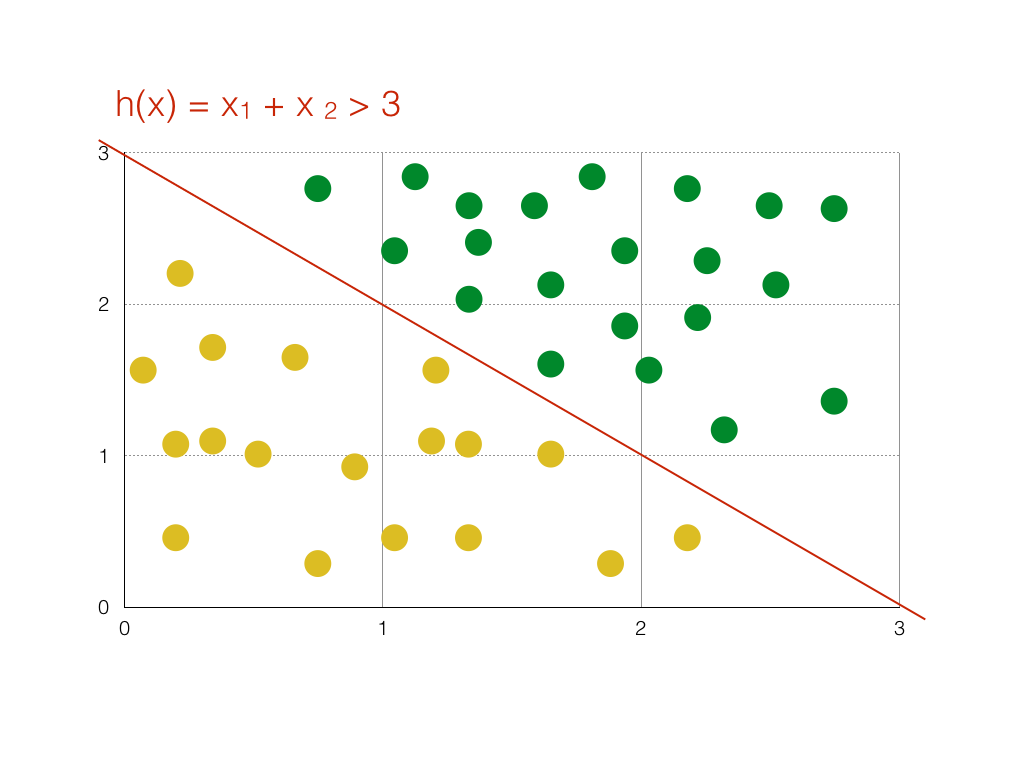
\includegraphics[height=6cm]{images/regression_logistique.png}
	\caption[Exemple d'une régression logistique]{Exemple d'une régression logistique. Les données en jaune sont séparées des données vertes par la frontière de décision (ligne rouge sur le graphe).}
	\label{fig:Exemple d'une regression logistique}
\end{figure}


\subsubsection{Ligne de décision non linéaire}
\label{Le Machine Learning: Les différents algorithmes: La regression logistique: Ligne de décision non linéaire}
Il est possible d'utiliser des hypothèses plus complexes, permettant d'effectuer de la classification non linéaire. \\
On a par exemple $h_\theta(x) = g(\theta_0+ \theta_1x_1 + \theta_2x_2 + \theta_1x_1^2 + \theta_1x_2^2)$ avec $\theta = \begin{blockarray}{[c]} -1 \\ 0 \\ 0 \\ 1 \\ 1 \end{blockarray}$.\\
 Cela revient à dire: 

\begin{equation}
\begin{split}
	y=1 \text{ si } -1 + x^2_1 + x^2_2 \ge 0 \\
	soit x^2_1 + x^2_2 \ge 1
\end{split}
\end{equation}

Cette frontière de décision correspond à l'équation d'un cercle. Plus le nombre de polynômes de l'hypothèse est important, plus on peut créer des lignes de décisions complexes. 

\subsubsection{Fonction coût}
\label{Le Machine Learning: Les différents algorithmes: La regression logistique: Fonction coût}
Dans le cadre d'une régression linéaire, la forme de l'hypothèse est linéaire. Pour la régression logistique, elle ne l'est plus (forme sigmoïde). La fonction coût n'est donc ici pas convexe (graphe convexe de la régression linéaire figure \ref{fig:Régression linéaire, calcul des paramètres de l'hypothèse}) et on ne peut pas déterminer le minimum global (et donc la valeur optimale des paramètres de l'hypothèse), celle-ci pouvant posséder plusieurs minimums locaux. Pour palier à ce problème, on s'appuie sur une reformulation de la fonction coût. \\
Soit la fonction coût utilisée pour la régression linéaire:
\begin{equation}
	J(\theta) = \frac{1}{m}\sum_{i=1}^{m}\frac{1}{2}(h_\theta(x^i)-y^i)^2
\end{equation}

On pose $Cost(h_\theta,y) = \frac{1}{2}(h_\theta(x^i)-y^i)^2$ le coût, on obtient:
\begin{equation}
J(\theta) = \frac{1}{m}\sum_{i=1}^{m}Cost(h_\theta,y)
\end{equation}

On reformule le coût dans le cadre de la régression logistique:
\begin{equation}
cost(h_\theta(x),y)=\begin{blockarray}{ll}
\begin{block}{\{ll}
-log(h_\theta(x)) & \text{ si } y=1 \\
-log(1 - h_\theta(x)) & \text{ si } y=0 \\
\end{block}
\end{blockarray}
\end{equation}

On peut réécrire cette formule en un seul bloc:
\begin{equation}
cost(h_\theta(x),y) = -ylog(h_\theta(x)) - (1-y)log(1-h_\theta(x))
\end{equation}

La fonction coût devient alors:
\begin{equation}
J(\theta) = \frac{1}{m}[\sum_{i=1}^{m}y^ilog(h_\theta(x))+(1-y^i)log(1-h_\theta(x^i))]
\end{equation}

Sous cette forme, la fonction coût est convexe. \\ \\

Intuitivement:
\begin{itemize}
	\item lorsque l'on observe la forme de la fonction $-log(h(\theta))$ (figure \ref{fig:fonctions -log(h(x)) et -log(1-h(x))}), vraie pour $y=1$, on remarque que lorsque $h(x)$ tend vers 1, le coût tend vers 0. Lorsque $h_\theta(x)$ tend vers 0, le coût tend vers l'infini. Autrement dit, plus la valeur de l'hypothèse s'approche de la valeur de sortie réelle (y=1), plus le coût est faible. Inversement, plus il s'en éloigne, plus il est élevé.
	\item Lorsque l'on observe la forme de la fonction $-log(1-h(\theta))$ (figure \ref{fig:fonctions -log(h(x)) et -log(1-h(x))}), vraie pour $y=0$, on remarque que lorsque $h(x)$ tend vers 0, le cout s'approche de 0. Lorsque $h_\theta(x)$ tend vers 1, le coût tend vers l'infini. Autrement dit, plus la valeur de l'hypothèse s'approche de la valeur de sortie réelle (y=0), plus le coût est faible et inversement, plus il s'en éloigne, plus il est élevé.
\end{itemize}
C'est le comportement que l'on attend de la fonction coût, i.e. optimiser l'hypothèse de manière à ce que celle-ci s'approche de la valeur de sortie réelle.

\begin{figure}[h]
	\centering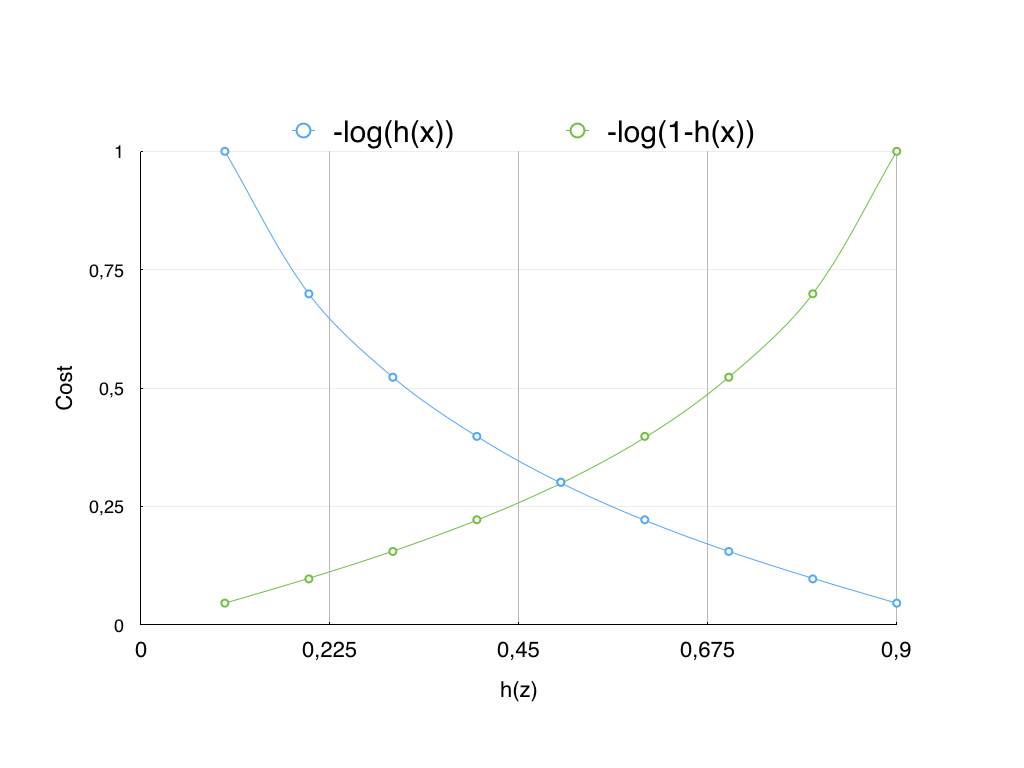
\includegraphics[height=8cm]{images/cost_log.png}
	\caption[fonctions $-log(h_\theta(x))$ et $-log_\theta(1-h(x))$]{fonctions $-log_\theta(h(x))$ et $-log_\theta(1-h(x))$}
	\label{fig:fonctions -log(h(x)) et -log(1-h(x))}
\end{figure}

\subsubsection{Algorithme du gradient}
\label{Le Machine Learning: Les différents algorithmes: La regression logistique: L'algorithme du gradient}
La formule de l'algorithme du gradient reste identique à celle utilisée pour la régression linéaire, seule la valeur de $h_\theta(x)$ change, selon la démarche soumise en partie \ref{Le Machine Learning: Les différents algorithmes: La regression logistique: Fonction coût}.

\begin{equation}
\begin{split}
\text{Repeat \{} \\
\theta_j = \theta_j - \alpha \frac{1}{m}\sum_{m}^{i=1}(h_\theta(x^i) - y^i)x_j^i \\
\text{\}} \\
\end{split}
\end{equation}

\subsubsection{Classification multiclasse}
\label{Le Machine Learning: Les différents algorithmes: La regression logistique: La classification multi-classe}
Les exemples de classification proposés jusqu'ici ne comportaient que deux classes. Or il est possible de résoudre des problèmes dont la décision doit être prise parmi plus de deux classes. Soit l'exemple de la prévision saisonnière (partie \ref{Le Machine Learning: Généralités sur le Machine Learning: Définition et principe général:un exemple concret}), on a en sortie une décision à prendre parmi les 4 classes: printemps, été, automne et hiver. Pour résoudre ce problème, on compare une classe par rapport à l'ensemble des autres classes (considérées alors comme un seul et même ensemble homogène). On répète ensuite le même procédé pour les autres classes. L'exemple analysé appartient à la classe ayant eu la probabilité la plus élevée en sortie. Cette méthode s'appelle la "One-vs-All".


\subsection{Support Vector Machine}
\label{Le Machine Learning: Les différents algorithmes: SVM}
Le Support Vector Machine (traduire en français par "Machine à vecteurs de support") permet de résoudre des problèmes de classification. Conceptuellement, le SVM reprend les théories appliquées à la régression logistique. On y ajoute deux notions supplémentaires: la marge maximale et les fonctions noyaux.

\subsubsection{Marge maximale}
\label{Le Machine Learning: Les différents algorithmes: SVM: la marge maximale}
Afin d'expliquer ce qu'est la notion de marge maximale, on s'appuie sur un exemple dans lequel les données sont séparables par une ligne de décision linéaire. Dans le cas de la figure \ref{fig:Svm: cas simple d'une regression logistique avec une hypothèse linéaire}, on a un problème de classification composé de deux classes. Le but est donc de déterminer une valeur de l'hypothèse permettant de séparer ces deux régions (représentée par la frontière de décision). On remarque qu'elle peut prendre une infinité de valeurs (i.e. il existe une infinité de combinaisons de valeurs des paramètres $\theta$ de l'hypothèse résolvant la classification). On cherche donc à déterminer l'hypothèse permettant de répondre de manière optimale à ce problème. Pour cela, on introduit la notion de marge. Comme on peut l'observer sur la figure \ref{fig:Svm: optimisation du calcul de l'hypothèse par l'introduction de marges}, la ligne de décision est bordée de deux marges. Celles-ci prennent appui sur les valeurs situées à l'extrémité de chacune des deux régions homogènes de données. Afin de déterminer la meilleure position pour la ligne de décision (et donc le paramétrage optimal de l'hypothèse), on maximise la distance entre ces deux marges. 

\begin{figure}[h]
	\centering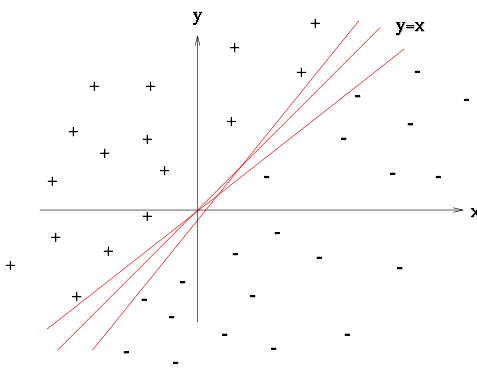
\includegraphics[height=6cm]{images/svm_no_margin.png}
	\caption[SVM: cas simple d'une régression logistique avec une hypothèse linéaire]{Svm: cas simple d'une régression logistique avec une hypothèse linéaire. On observe sur la figure ci-contre qu'il existe une infinité de positions de la frontière de décision délimitant les deux classes. Cependant la performance de chacune d'elle peut être différente.}
	\label{fig:Svm: cas simple d'une regression logistique avec une hypothèse linéaire}
\end{figure}

\begin{figure}[h]
	\centering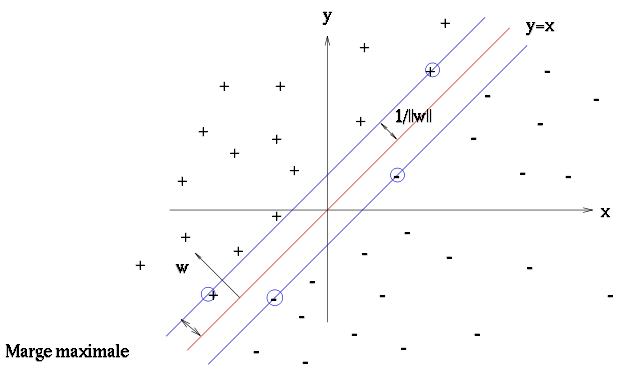
\includegraphics[height=6cm]{images/svm_margin.png}
	\caption[SVM: optimisation du calcul de l'hypothèse par l'introduction de marges]{Svm: optimisation du calcul de l'hypothèse par l'introduction de la notion de marges. Afin de déterminer la position optimale pour la frontière de décision, on introduit deux marges entres les échantillons à l'extrémité des classes et la ligne de décision. On cherche à maximiser la distance entre ces deux marges afin d'obtenir la frontière de décision optimisant la classification.}
	\label{fig:Svm: optimisation du calcul de l'hypothèse par l'introduction de marges}
\end{figure}

\subsubsection{Les fonctions noyaux}
\label{Le Machine Learning: Les différents algorithmes: SVM: les fonctions noyaux}
Les fonctions noyaux (également appelées Kernel) permettent de résoudre des problèmes de classifications non linéaires grâce à des méthodes de classifications linéaires. Pour cela, on transforme l'espace de représentation des données d'entrées en un espace de plus grande dimension dans lequel il est possible de délimiter les classes par une frontière de décision linéaire (figure \ref{fig:Svm: Exemple d'un problème de classification linéaire} et \ref{fig:Svm: Exemple d'un problème de classification non linéaire}) .

\begin{figure}[h]
	\centering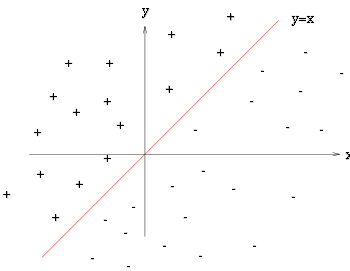
\includegraphics[height=6cm]{images/svm_regression.png}
	\caption[Exemple d'un problème de classification linéaire]{Exemple d'un problème de classification linéaire. On observe qu'ici les deux classes (+ et -) sont séparables par une frontière de décision linéaire. }
	\label{fig:Svm: Exemple d'un problème de classification linéaire}
\end{figure}

\begin{figure}[h]
	\centering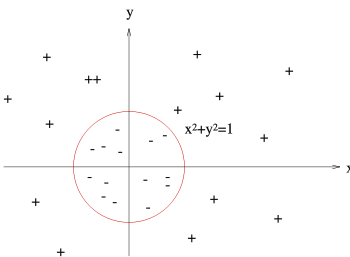
\includegraphics[height=6cm]{images/svm_cercle.png}
	\caption[Exemple d'un problème de classification non linéaire]{Exemple d'un problème de classification non linéaire. On observe que les deux classes (+ et -) ne sont pas linéairement séparables. Pour résoudre ce problème, on utilise des kernels afin de modifier l'espace de représentation et trouver un espace où il est possible de résoudre le problème par une frontière linéaire.}
	\label{fig:Svm: Exemple d'un problème de classification non linéaire}
\end{figure}

\subsubsection{Avantages du SVM}
\label{Le Machine Learning: Les différents algorithmes: SVM: Avantage du SVM}
L'entrainement d'un algorithme de type SVM peut être effectué avec peu d'exemples. En effet, la marge maximale s'appuie sur les données en périphéries des ensembles homogènes. De plus, il s'agit d'un outil puissant et facilement adaptable.

\subsection{Périmètres d'utilisation de la régression logistique et du SVM}
\label{Le Machine Learning: Choix de la méthode à utiliser: Comparaison de la régression logistique et le SVM}
La régression logistique et le SVM sont tous deux des algorithmes de classification. Le choix d'un modèle dépend du nombre d'exemples que l'on a pour l'entrainement et du nombre de features. On présente dans le tableau \ref {tab:Périmètre d'utilisation de la régression logistique et le SVM} les différents périmètres d'utilisation.

\begin{table}[h]
	\begin{tabular}{ | p{7cm} | p{7cm} |}
		\hline
		Périmètres d'utilisation & Modèle d'apprentissage à favoriser \\
		\hline 
		le nombre de features est plus important que le nombre d'exemples (environ 1000 features pour 10 à 100 exemples) & Régression logistique ou SVM sans kernel \\
		\hline
		le nombre de features est faible (1 à 1000 features pour 10 à 10 000 exemples) & SVM avec un kernel \\
		\hline 
		si le nombre de features est faible et le nombre d'exemples élevé ( 1 à 10 000 features pour 50 000 à 1 million d'exemples) & Régression logistique ou svm sans kernel avec création de features. \\
		\hline
	\end{tabular}
	\caption[Périmètre d'utilisation de la régression logistique et le SVM]{Périmètre d'utilisation de la régression logistique et le SVM}
	\label {tab:Périmètre d'utilisation de la régression logistique et le SVM}
\end{table}

\subsection{Autres algorithmes  d'apprentissage supervisé}
\label{Le Machine Learning: Choix de la méthode à utiliser: Autres algorithmes pour l'apprentissage supervisé}
Les méthodes proposées jusqu'ici ne représentent qu'un échantillon du parc algorithmique constituant l'apprentissage automatique supervisé. On peut notamment évoquer les réseaux neuronaux qui sont des algorithmes puissants et sont beaucoup utilisés dans le traitement et l'analyse d'images (mais requièrent un nombre d'exemples élevé). On peut également mentionner les arbres de décision (e.g. Markov).